\chapter{Implementierung}

\section{Einleitung}

Ziel dieser Arbeit war es, eine Implementierung von Sensoren in eine Simulationsumgebung zu integrieren. Es sollte viele verschiedene Arten von Sensorknoten geben, die jeweils einen oder mehrere verschiedene Sensoren besitzen. Mit diesen Knoten sollte es möglich sein, ein Netzwerk aufzubauen, um die Umgebungsparameter eines ganzen Gebietes zu erfassen.
Die Daten der Simulation sollten visualisiert und ausgewertet werden können, besonders hinsichtlich Energieverbrauch und den dazugehörigen Batteriezuständen der jeweiligen Elemente im Verlauf der Zeit.

\section{Aufbau und Struktur}

\subsection{Klassenübersicht}

Die Klassenübersichten wurden teilweise mit Hilfe von doxygen\cite{doxygen} erstellt. Die Tabelle \ref{Klassenübersicht} zeigt einen Überblick über die definierten Module.

\begin{table}[!ht]
  \centering
  \caption{Klassenübersicht}
  \label{Klassenübersicht}
\begin{tabularx}{\textwidth}{ll}
	\toprule
	Klasse & Beschreibung \\
	\midrule\midrule
	BatteryAccess &	\specialcell{gibt einer Klasse, welche von dieser erbt Zugriff auf \\die Batterie} \\\midrule
Memory & \specialcell{eine einfache Implementierung eines \\key-value-Speichers mit CRUD-Operationen}\\\midrule
Processor	& \specialcell{Repräsentiert ein paar Grundfunktionen eines \\ Prozessor übernimmt die Steuerung der Sensoreinheit, \\ hat Zugriff auf den Speicher und  kann \\außerdem zwischen verschiedenen power-Modi wechseln }\\\midrule
AbstractSensingUnit & \specialcell{einfache Implementierung einer SensingUnit \\ diese kann Werte der Umgebung messen und \\verbraucht dabei Energie}\\\midrule
SensorNode	& \specialcell{ist hauptsächlich für die Initialisierung zuständig}\\\midrule
AbstractSignalConditioner	& modelliert den Energieverbrauch vom SignalConditioner \\\midrule
AbstractSignalConverter	& modelliert den Energieverbrauch vom SignalConverter\\\midrule
AbstractTransducer	& modelliert den Energieverbrauch vom Transducer\\\midrule
CustomWorldUtility	& \specialcell{stellt die Umgebung dar:\\ generiert Umweltparameter und speichert diese\\ liefert auf Anfrage von Sensoren Messwerte}\\\midrule
ExtendedMessage & Nachricht mit einigen Parameters für Statistiken\\\midrule
SimpleSensorData	& \specialcell{eine Klasse die von cNamedObject erbt\\ kann eingesetzt werden um an die Parameterliste \\von Nachrichten angehängt zu werden\\mit dieser können Integerwerte versendet werden}\\\midrule
StatisticsInterface & Interface welches Statistiken zur Verfügung stellt\\
	\bottomrule
\end{tabularx}
\end{table}

\subsubsection{CustomWorldUtility}

Die Klasse CustomWorldUtility ist eine sehr wichtige für die Simulation. Sie repräsentiert die Umgebung, also den Bereich, indem sich die Knoten befinden. Sie erbt von der Klasse BaseWorldUtility aus dem MiXiM-Framework. BaseWorldUtility stellt die nötigen Funktionalitäten für den sogenannten Playground bereit. \newline
Zusätzlich dazu stellt die Klasse selbst die notwendigen Parameter für die Umwelt bereit. Nach dem Starten der Simulation steht darin jeweils ein k-dimensionales Array pro Sensortyp bereit: temperatureArray, pressureArray, humidityArray und lightArray. Dabei ist k die definierte Anzahl der Dimensionen, je nachdem ob eine 2-dimensionale Fläche oder ein 3-dimensionaler Raum simuliert werden soll. Die Arrays enthalten die Parameter der Umgebung; temperatureArray beinhaltet zum Beispiel, wie der Name schon sagt, Informationen über die Temperatur. \newline
Es kann zu Beginn der Simulation entschieden werden, ob neue Werte berechnet werden sollen oder die bereits vorhandenen Werte für die Umgebung übernommen werden sollen. Die Arrays besitzen die gleiche Größe wie der Playground. Diese Größe ist auch zusätzlich in den Parametern sizeX, sizeY und sizeZ gespeichert. \newline
Da jedoch im 3-dimensionalen Fall die Datenmenge sehr schnell steigt, ist auch möglich über den Paremeter dataGranularity im zugehörigen ned-Modul zu definieren, wie detailliert die Daten erstellt werden sollen. Sollte man zum Beispiel den Wert 10 setzen, so wird nur alle 10 Meter ein Wert generiert.\\
Wenn neue Werte generiert werden sollen, so wird für jeden Messtyp eine xml-Datei in der entsprechenden Größe angelegt und mit Messdaten gefüllt. Diese werden anschließend ausgelesen und in Form der oben genannten Arrays gespeichert. Wenn keine neuen Daten erstellt werden sollen, so wird ein bereits existierendes xml-File genutzt.\\
Zum Erstellen neuer Daten kann die Funktion generateEnvironmentData() genutzt werden. Es ist dadurch auch möglich während der Simulation neue Werte zu generieren, indem man diese Funktion aufruft. Die Funktion legt pro Umweltparameter eine xml-Datei im Ordner \textit{WorldModel/data} an. Jede der xml-Dateien wird beim Start mithilfe der Funktion readXML(int) eingelesen, verarbeitet, das heißt in ein Array umgewandelt und anschließend in der Klasse gespeichert. \newline
Sollte nun ein Sensor einen Messwert auslesen wollen, so kann dieser auf die Funktion getValueByPosition((std::string type, Coord *position)) zugreifen und anhand seines Sensortyps und seiner Position einen entsprechenden Wert geliefert bekommen.

\paragraph{Einblick in einige Funktionen}

Wie im vorigen Abschnitt beschrieben, übernimmt die Funktion generateEnvironmentData() das Erstellen von Umweltparametern. Dafür ruft sie, je nach Sensordatentyp, eine der folgenden Funktionen auf:

\begin{multicols}{2}
\begin{itemize}
\item generateTemperature() - $^\circ $C
\item generatePressure() - hPa
\item generateHumidity()- \%
\item generateLight() - lx
\end{itemize}
\end{multicols}

Diese Funktionen generieren je ein 2- oder 3-dimensionales Array in der Größe des Playgrounds mit Werten, die die jeweils oben angegebenen Einheiten besitzen. In Listing \ref{lst:generateTemp} ist die generateTemperature()-Funktion als ein Beispiel aufgeführt. Im Falle dieser Funktion werden Zufällige integer-Werte generiert, welche sich im Bereich 10 bis 30 bewegen. Dieser erste Entwurf ermöglicht es erst einmal, dass einfach und halbwegs realitätsnahe Werte für den jeweiligen Umweltparameter vorliegen. Später kann an dieser Stelle dann auch ein Zugriff auf eine externe Datenbank erfolgen, in der Messwerte gespeichert sind, die in einem realen Gebiet gemessen wurden.

\begin{lstlisting}[language=C++, label=lst:generateTemp, caption=generateTemperature()]
int* CustomWorldUtility::generateTemperature(int size)
{
    int* data = new int[size];
    for (int i = 0; i < size; i++) {
        //10 - 30
        data[i] = (int)((rand() % 100)/5) + 10;
    }
    return data;
}
\end{lstlisting}

\begin{lstlisting}[language=C++, label=lst:readXML, caption=Kurzbeschreibung readXML()]
cXMLElementList nListRows = rootE->getChildren();
int count = nListRows.size();
for (int i = 0; i < count; i++){
    val[i] = atoi(nListRows[i]->getNodeValue());
}
\end{lstlisting}

Um eben diese Daten wieder lesen zu können, dient die Funktion readXML(). Sie verwendet die cXMLElement-Funktionen aus dem Omnet++-Framework. Diese sind sehr hilfreich beim Verarbeiten von XML-Dateien. Ein Beispiel für die Verwendung bei einem XML-File mit einer Verschachtelungstiefe von 1 ist im Listing \ref{lst:readXML} zu sehen. Da in dieser Simulation die Umweltparameter in Form von XML gespeichert sind, ist dies eine sehr nützliche Funktionalität.\\
Die bis jetzt beschriebenen Funktionen dienen alle zur Initialisierung der Simulationsdaten. Es ist natürlich auch möglich diese in einem späteren Verlauf der Simulation erneut aufzurufen und damit neue Werte zu generieren. \\
Für den späteren Verlauf der Simulation ist nun noch die Funktion getValueByPosition(std::string, Coord*) (\ref{lst:getValueByPosition}) von großer Bedeutung. Diese Funktion ermöglicht den Sensoreinheiten, auf die gespeicherten Daten zuzugreifen.

\begin{lstlisting}[language=C++, label=lst:getValueByPosition, caption=getValueByPosition()]
int CustomWorldUtility::getValueByPosition(std::string type, Coord *position)
{
    int*** data = readXML(getEnumFromType(type));
    int dataAtPosition =
            data
                [(int)(position->x/par("dataGranularity").longValue())]
                 [(int)(position->y/par("dataGranularity").longValue())]
                  [(int)(position->z/par("dataGranularity").longValue())];
    return dataAtPosition;
}
\end{lstlisting}

\subsubsection{SensorNode}

Die Klasse AbstractSensorNode selbst enthält eher weniger Funktionalität. Sie dient hauptsächlich zum Initialisieren des gesamten Knotens. Das funktioniert in Omnet++ natürlich zum größten Teil automatisch, allerdings liegt für die Sensoren eine parameterabhängige, generische Initialisierung vor. So können innerhalb des NED-Moduls die folgenden boolschen Parameters gesetzt werden:
\begin{itemize}
\item hasTemperatureSensor
\item hasHumiditySensor
\item hasPressureSensor
\item hasLightSensor
\end{itemize}
Je nachdem ob der jeweilige Parameter gesetzt wird oder nicht, wird das entsprechende Sensormodul auf dem Sensorknoten erstellt. Die Gates und Connections eines Moduls lassen sich in der NED-Definition leider nicht so schön generisch erstellen.\\
Daher wird die Initialisierung des Prozessors zusammen mit seinen Gates, Connections und den entsprechenden Channels in der C++-Klasse übernommen. Nach dem Erstellen des Prozessors selbst werden für jeden existierenden Sensor ein eingehendes und ein ausgehendes Gate erstellt. Zusätzlich wird noch ein beidseitiges Gate für die Verbindung zum Memory-Modul angelegt.\\
Die Prozessorgates erhalten dann die Verbindungen zu den jeweils entsprechenden Gates, zum Sensor verläuft ein Gate zur Sensing Unit, das vom Sensor eingehende kommt vom Transducer. Beide Verbindungen haben unterschiedliche Funktionen, einmal lediglich zum Senden eines Signals um innerhalb der Sensing Unit einen Messvorgang gestartet und ein anderes Mal um die gemessenen Werte an den Prozessor zu übermitteln. Es wird daher in 2 verschiedene Channels zum Senden unterschieden, welche entsprechend eine höhere oder niedrigere Datenrate aufweisen können, je nachdem wie diese innerhalb des ini-Files definiert sind.\\
Wie genau der Prozessor Schritt für Schritt angelegt wird, ist im Listing \ref{lst:initProc} zu sehen. Für das Beispiel wurde jedoch nur ein Paar von Gates verbunden, da die Verbindung für alle anderen Gates analog aussieht.

\begin{lstlisting}[language=C++, label=lst:initProc, caption=teilweise Initialisierung des Prozessors]
//get processor module type
cModuleType *moduleType = cModuleType::get("sensortechnology.src.SensorNode.Processor.Processor");
//create module
cModule *processor = moduleType->create("Processor", this);
processor->finalizeParameters();
//create gate
cGate *fromSensor = processor.addGate(("from" + SensorType + "Sensor").c_str(), cGate::INPUT);
//get sensor
cModule *Sensor = this->getSubmodule((SensorType + "Sensor").c_str());
//get sensor gate
cGate *sensorOut = Sensor->gate("fromTransducerToNodeProcessor");    
//connect the gates
sensorOut->connectTo(fromSensor);    
//finish the process
processor->buildInside();
\end{lstlisting}

\subsubsection{Sensormodule}

Der Sensor in seiner Gesamtheit besitzt keine eigene C++-Klasse. Jedoch besitzt er 4 Module, die gemeinsam die Funktionalität des Sensors ausmachen, welche jeweils eine Klasse haben. Diese werden im folgenden Abschnitt beschrieben.

\paragraph{SensingUnit}

Die SensingUnit ist der wichtigste Teil des Sensors. Innerhalb der Definition von handleMessage(cMessage*) wartet das Modul auf ein Signal vom Prozessor. Sobald dieses kommt, wird ein Messvorgang gestartet. Zunächst überprüft das Modul dabei die eigene Position. In Abhängigkeit von dieser wird anschließend ein dem Typ entsprechender Messwert aus dem Modul CustomWorldUtility ausgelesen, welcher hinterher an den SignalConditioner weitergegeben wird. Dazu wird eine Instanz der Klasse SimpleSensorData genutzt, welche an eine cMessage angehängt wird und dann über das entsprechende Gate gesendet wird.

\paragraph{SignalConditioner}

Der SignalConditioner wartet auf eingehende Daten von der SensingUnit. In der Praxis würde das Signal hier aufbereitet werden, jedoch ist die genaue Modellierung an dieser Stelle nicht relevant. Daher kann lediglich ein Energieverbrauch für die durchgeführten Operationen definiert werden, welcher dann bei jedem Aufruf verbraucht wird. Anschließend werden eingegangene Nachrichten weitergeleitet an den SignalConverter.

\paragraph{SignalConverter}

Für den SignalConverter gilt dasselbe wie für den SignalConditioner. Die eingegangenen Nachrichten werden lediglich an den Transducer weitergeleitet, ohne das genaue Verhalten zu simulieren und auch dabei steht wieder nur die Modellierung des Energiehaushalts im Vordergrund. 

\paragraph{Transducer}

Das letzte Bauteil der Messkette ist der Transducer. Dieser erhält seine Daten vom SignalConverter. Auch hier steht der Energieverbrauch im Vordergrund. Wie in der Realität auch, hat der Transducer am Ende den verwertbaren Messwert in einer festgelegten Einheit vorliegen. Dieser wird anschließend an den Prozessor gesendet, welcher sich dann um die Verwendung dessen kümmert.

\subsubsection{Prozessor}

Eine wichtige Funktion des Prozessors wurde eben schon indirekt beschrieben. Die Klasse Processor kümmert sich um die Steuerung des Sensors. Aber er erfüllt auch andere Funktionen, wie die Energieverwaltung des Sensorknotens und die Verwertung von statistischen Daten.

\paragraph{Sensorsteuerung}

Der jeweilige Prozessor kann über das entsprechende, ausgehende Gate zu seinen Sensoren einen Messvorgang auslösen, indem die Funktion startSensingUnit() (Listing \ref{lst:startSensingUnit}) aufgerufen wird. Anschließend bekommt er die Daten vom Transducer übermittelt. Diese Information kann nun unterschiedlich behandelt werden. Typischerweise kann dieser Wert nun zunächst im Speicher hinterlegt werden. Dafür wird die eingegangene Message direkt an den Memory weitergeleitet. Wie das genau aussieht, ist im folgenden Abschnitt des Memories beschrieben.\\
Es ist auch möglich, periodisch Messungen durchzuführen. Dazu muss lediglich im NED-Modul ein Wert für sensingIntervall gesetzt werden. Dieser legt fest, welche zeitlichen Abstände zwischen 2 Messungen vorliegen sollen. Es wird dann bei der Initialisierung ein Event gestartet, welcher jeweils nach dem festgelegten Zeitintervall ausgelöst wird. In diesem Fall wird dann ein Messvorgang gestartet. Danach wird der nächste folgende Event initialisiert und zum gegebenen Zeitpunkt beginnt der Vorgang von Neuem.

\begin{lstlisting}[language=C++, label=lst:startSensingUnit, caption=startSensingUnit()]
void Processor::startSensingUnit()
{
    cModule* SensorNode = getParentModule();
    if (SensorNode->par("hasTemperatureSensor")) {
        cMessage* msg = new cMessage("startMeasuring");
        send(msg, "toTemperatureSensor");
    }
    if (SensorNode->par("hasHumiditySensor")) {
        cMessage* msg = new cMessage("startMeasuring");
        send(msg, "toHumiditySensor");
    }
    if (SensorNode->par("hasPressureSensor")) {
        cMessage* msg = new cMessage("startMeasuring");
        send(msg, "toPressureSensor");
    }
    if (SensorNode->par("hasLightSensor")) {
        cMessage* msg = new cMessage("startMeasuring");
        send(msg, "toLightSensor");
    }
}
\end{lstlisting}

\paragraph{ProcessorMode}

Weiterhin hat der Prozessor die Möglichkeit zwischen verschiedenen Powermodi zu wechseln. Die existierenden Modi sind in einem enum (Listing \ref{lst:ModeEnum}) definiert und können per Funktion switchProcessorMode gewechselt werden (Listing \ref{lst:switchProcessorMode}).

\begin{lstlisting}[language=C++, label=lst:ModeEnum, caption=enum MODES]
enum MODES { 
	NORMAL = 0, 
	POWER_SAVING = 1, 
	HIGH_PERFORMANCE = 2, 
	OFF 
}
\end{lstlisting}

\begin{lstlisting}[language=C++, label=lst:switchProcessorMode, caption=switchProcessorMode()]
void Processor::switchProcessorMode(MODES mode)
{
    //switch batteries power accounts
    if (mode == POWER_SAVING) {
        drawCurrent(currentOverTimePowerSaving, 1);
    } else if (mode == NORMAL) {
        drawCurrent(currentOverTimeNormal, 0);
    } else if (mode == HIGH_PERFORMANCE) {
        drawCurrent(currentOverTimeHighPerformance, 2);
    }
}
\end{lstlisting}

So können beispielsweise Wach-und-Schlaf-Zyklen der Sensorknoten gesteuert werden. Da die Energiequelle von Sensorknoten oft sehr klein ist, ist es sinnvoll die Knoten in Zeiten, in denen keine Messwerte aufgenommen werden sollen in einen Stand-by Zustand zu versetzen. Dadurch kann viel Energie gespart werden.\\
Diese Funktion wird durch die verschiedenen Powermodi bereitgestellt. Es ist möglich einen Zeitintervall zu definieren, in dem die verschiedenen Knoten gemeinsam zwischen den verschiedenen Modi wechseln. Da ein Knoten in Zeiten des Stand-by keine Kommunikation durchführen kann, ist am sinnvollsten alle Knoten im Netzwerk synchron schlafen zu lassen. Der entsprechende Zeitintervall kann durch die Variable shiftProcessorModeIntervall definiert werden.\\
Dadurch werden nun wieder zeitlich periodische Wechsel zwischen den Modi durchgeführt, welche durch Events gesteuert werden, indem die Funktion switchProcessorMode() (\ref{lst:switchProcessorMode}) aufgerufen wird. Diese Funktion ist überladen und kann auf 3 verschiedene Arten aufgerufen werden: mit dem Modus in die gewechselt werden soll, mit dem int-Wert der diesen Modus repräsentiert oder ohne Parameter, in dem Fall wird der nächste Modus anhand der Integerwerte bestimmt, wie bei einem Modulozähler.\\
Für jeden einzelnen Zustand kann dann wiederum im ini-File definiert werden, wie der Energieverbrauch pro Zeiteinheit während welches Modus genau aussehen muss.

\paragraph{Statistiken}

Die dritte Funktion des Prozessors, welche ebenfalls über Events gesteuert wird, ist das Erfassen statistischer Daten. Auch hierfür kann, in Form von der Variable collectStatisticsIntervall, ein zeitlicher Intervall definiert werden, nach diesem jeweils ein Event eine Erhebung von statistischen Messwerten des Batteriezustands durchführt. Die dazu gehörige Funktion ist in Listing \ref{lst:doCollectStatistics} zu sehen.

\begin{lstlisting}[language=C++, label=lst:doCollectStatistics, caption=doCollectStatistics()]
void Processor::doCollectStatistics()
{
    voltage = battery->getVoltage();
    voltageStats.collect(voltage);
    voltageVector.record(voltage);

    residualRelative = battery->estimateResidualRelative();
    residualRelativeStats.collect(residualRelative);
    residualRelativeVector.record(residualRelative);

    residualAbs = battery->estimateResidualAbs();
    residualAbsStats.collect(residualAbs);
    residualAbsVector.record(residualAbs);
}
\end{lstlisting}

Mit Abbildung \ref{fig:switchingModes5000} ist ein Beispiel gegeben, bei dem alle 3 Events in Verwendung waren. Dabei ist natürlich von der Sensorsteuerung nicht viel zu sehen. Alle 5000 Sekunden wurde hierbei der Modus gewechselt, beginnend bei dem normalen Modus, danach einem energiesparenden Modus und zuletzt einem Modus mit sehr hohem Energieverbrauch. Danach wieder beginnend von vorn. Dabei wurde alle 1000 Sekunden der Ladezustand abgefragt. Diese Operationen wurden auf 4 verschiedenen Sensorknoten parallel durchgeführt. Man kann sehr gut sehen, dass der gelbe Verlauf besonders schnell nach unten geht. Das liegt daran, dass dort ein Knoten mit 4 Sensoren genutzt wurde. Der Rote dagegen konnte deutlich länger am Leben bleiben, weil dieser Knoten lediglich einen Temperatursensor besaß. Der Energieverbrauch für die jeweils analogen Bauteile war bei allen 3 Sensorknoten gleich.

\begin{figure}[htbp]
\centering
\caption{Beispielstatisik Relativer Batterieladezustand}
\label{fig:switchingModes5000}
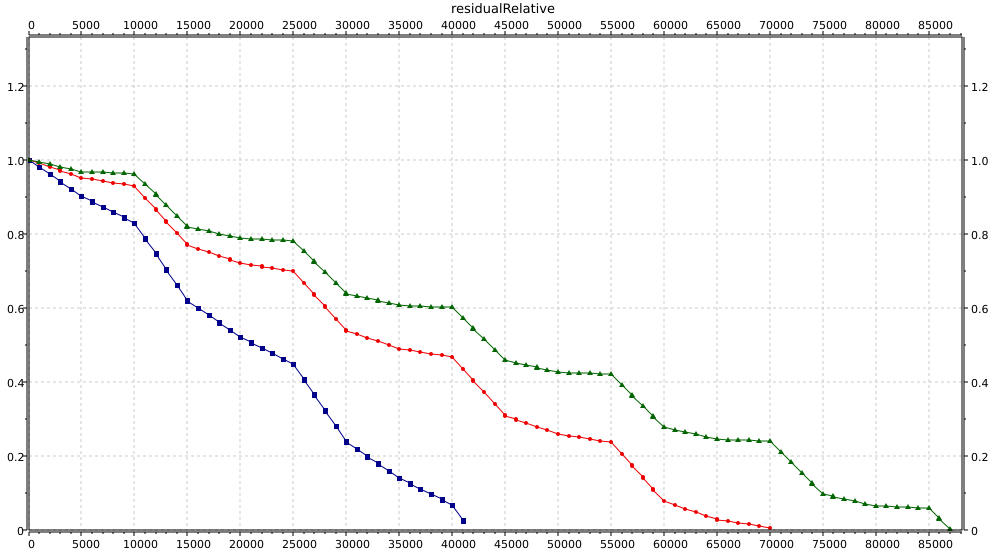
\includegraphics[width=\textwidth]{switchingModes5000}
\end{figure}

\subsubsection{Memory}

Der Speicher besitzt Arrays für einen key-value-Speicher und implementiert zur Benutzung dieses Speichers die CRUD-Operationen, wie in Listing \ref{lst:CRUD} zu sehen ist.

\begin{lstlisting}[language=C++, label=lst:CRUD, caption=CRUD-Operationen vom Memory]
#define error -9999
const static int storageSize = 4;

void Memory::createEntry(std::string type, int value)
{
    int emptyId = -1;
    for (int i = 0; i < storageSize; i++) {
        if (storageType[i] == "") {
            emptyId = i;
            break;
        }
    }
    if (emptyId == -1) {
        return;
    }
    storageType[emptyId] = type;
    storageValue[emptyId] = value;
}

int Memory::readEntry(std::string type)
{
    int id = getIdByType(type);
    if (id == -1) {
        return error;
    }
    return storageValue[id];
}

void Memory::updateEntry(std::string type, int value)
{
    int id = getIdByType(type);
    if (id == -1) {
        return createEntry(type, value);
    }
    storageValue[id] = value;
}

void Memory::deleteEntry(std::string type)
{
    int id = getIdByType(type);
    if (id == -1) {
        return;
    }
    storageValue[id] = error;
    storageType[id] = "";
}
\end{lstlisting}

Wenn nun von außen eine Message mit einem Datensatz an den Speicher geschickt wird, so kann dieser je nach Bedarf Datensätze neu anlegen, löschen oder updaten, damit diese später, wenn die Daten benötigt werden, wieder abgerufen werden können.

\subsubsection{BatteryAccess}

Die Klasse BatteryAccess ermöglicht den Modulen des Sensors auf die Batterie zugreifen zu können. Dafür ist zunächst eigentlich die Klasse MiximBatteryAccess zuständig. BatteryAccess erbt von dieser und erweitert sie um einige wichtige Funktionen.\\
So können zum Beispiel direkt Werte für den Energieverbrauch des entsprechenden Moduls hinterlegt werden. Immer wenn nun eine energieintensive Operation durchgeführt wird, verbraucht die Batterie Energie in Höhe dieses definierten Wertes, indem die Funktion draw() aufgerufen wird. Diese ruft anschließend die Funktion drawEnergie(float) mit dem gespeicherten Wert float energiePerOperation auf. \\
Die Klasse kümmert sich weiterhin um die Initialisierung und um den Fall, dass die Batterie den leeren Zustand erreicht (handleHostState()).

\begin{lstlisting}[language=C++, label=lst:BatteryAccess, caption=BatteryAccess]
class BatteryAccess : public MiximBatteryAccess {
protected:
    float currentOverTime;
    float energiePerOperation;
    //int deviceID; - defined inside MiximBatteryAccess
public:
    BatteryAccess();
    virtual ~BatteryAccess();
    void initialize(int stage);
    void draw();
    void finish();
    virtual void handleHostState(const HostState &state);
};
\end{lstlisting}

\subsubsection{SimpleSensorData}

Die Klasse SimpleSensorData dient dazu, die Übertragung von Sensordaten zu ermöglichen. In Omnet++ ist es möglich, eine Parameterliste an Nachrichten anzuhängen. Die möglichen Parameter sind dabei eingeschränkt. Um nach dem Einfügen auch wieder auf die Parameter zugreifen zu können, wird cNamedObject als Parameter benötigt. Das ermöglicht beim späteren Auslesen des Parameters den Zugriff per string.\\
Es ist also nicht möglich, die C++-build-in-types direkt anzuhängen. Darum wird die Klasse SimpleSensorData genutzt, um die Integerwerte von Messungen per Nachricht zu übertragen.

\begin{figure}[htbp]
\centering
\caption{SimpleClasses: Member}
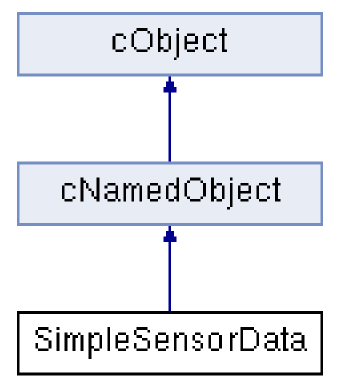
\includegraphics{SimpleClasses}
\end{figure}

\begin{minipage}{\textwidth}
\begin{lstlisting}[language=C++, label=lst:SimpleExample, caption=Beispiel für Senden und Empfangen mit Parameterliste]
//im Sender:
cMessage *msg = new cMessage(msgname);
SimpleSensorData *data = new SimpleSensorData("Temperature", temp);
msg->getParList().add(coord);

//
// Nachricht uebertragen    
//  
  
//im Empfaenger:  
SimpleSensorData *data = (SimpleSensorData*) msg->getParList().remove("Temperature");
\end{lstlisting}
\end{minipage}
\subsubsection{ExtendedMessage}

ExtendedMessage erbt direkt von der Klasse cMessage, der Standard-Nachrichtenklasse in Omnet++. Im Grunde stellt cMessage alle benötigten Funktionen bereit. ExtendedMessage ist nur aus dem Grund vorhanden, um zusätzliche Statistiken über Nachrichten erstellen zu können, zum Beispiel wie oft eine einzelne Nachricht weitergesendet wurde.

\begin{figure}[htbp]
\centering
\caption{ExtendedMessage: Vererbung}
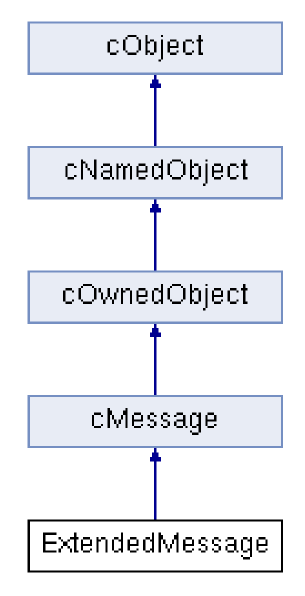
\includegraphics{ExtendedMessage}
\end{figure}

Im Listing \ref{lst:ExtendedMessage} ist zu sehen welche Statistikparameter erhoben werden.

\begin{minipage}{\textwidth}
\begin{lstlisting}[language=NED, label=lst:ExtendedMessage, caption=ExtendedMessage]
message ExtendedMessage extends cMessage
{
    int source;
    int destination;
    int hopCount = 0;    
}
\end{lstlisting}
\end{minipage}

\subsubsection{StatisticsInterface}

Dieses Interface enthält grundlegende Attribute für Statistiken. Klassen, die dieses implementieren, speichern somit zum Beispiel, wie viele Nachrichten sie empfangen oder gesendet haben. 

\subsection{Übersicht NED-Module}

Im folgenden Abschnitt werden alle Simulationsobjekte erläutert, also all jene, die durch die Sprache NED beschrieben wurden:

\begin{minipage}{\textwidth}
\begin{itemize}{\label{enum:NedModules}}
\item Simple Module
\begin{multicols}{2}
\begin{itemize}
\item AbstractSensingUnit
\item AbstractSignalConditioner
\item AbstractSignalConverter
\item AbstractTransducer
\item CustomWorldUtility
\item ExampleProcessor
\item Memory
\item Processor
\item SensingUnitHumidity
\item SensingUnitLight
\item SensingUnitPressure
\item SensingUnitTemperature
\item SignalConditionerHumidity
\item SignalConditionerLight
\item SignalConditionerPressure
\item SignalConditionerTemperature
\item SignalConverterHumidity
\item SignalConverterLight
\item SignalConverterPressure
\item SignalConverterTemperature
\item TransducerHumidity
\item TransducerLight
\item TransducerPressure
\item TransducerTemperature 
\end{itemize}
\end{multicols}
\item Compound Module
\begin{multicols}{2}
\begin{itemize}
\item AbstractSensor
\item SensorNode
\item HumiditySensor
\item LightSensor
\item PressureSensor
\item TemperatureSensor 
\end{itemize}
\end{multicols}
\item Messages und Channel
\begin{multicols}{2}
\begin{itemize}
\item ExtendedMessage
\item DatarateChannel
\end{itemize}
\end{multicols}
\item Network
\begin{multicols}{2}
\begin{itemize}
\item BasicWSN
\end{itemize}
\end{multicols}
\end{itemize}
\end{minipage}

\subsubsection{Simple Module}

Simple Module sind Komponenten in einer Omnet++ Simulation, die die größte Auswirkung auf die Wirkungsweise des Netzwerkes haben. Das liegt daran, dass bei ihnen neben einer Beschreibung in NED auch eine Beschreibung in C++ vorliegt. Daher kann das Verhalten jener Module während der Simulation ausführlich definiert werden. Simple Module werden oft in Gruppen zusammengefasst, also in Compound Modulen. Dadurch kann man komplexe Modellbeschreibungen erzeugen.\\
Im folgenden Teil werden einige dieser Simple Module beschrieben.

\subsubsection{CustomWorldUtility}

Wie im Codebeispiel (\ref{lst:CustomWorldUtility}) zu sehen ist, ist das Modul CustomWorldUtility eine Erweiterung des Moduls BaseWorldUtility. Zusätzlich zu den darin definierten Eigenschaften hat es einige weitere Parameter. Zum einen den integer-Wert dataGranularity, welcher festlegt, wie genau die Messwerte generiert werden sollen. Er legt fest, wie groß die Fläche, beziehungsweise der Würfel sein soll, für die jeweils ein Messwert angelegt wird. Dabei definiert dataGranularity die Kantenlänge. Die restlichen Variablen speichern die Speicherorte für die Messwerte, welche als xml-Datei erstellt werden.

\begin{minipage}{\textwidth}
\begin{lstlisting}[language=ned,caption={CustomWorldUtility},label=lst:CustomWorldUtility]
package mynetwork.WorldModel;
import org.mixim.base.modules.BaseWorldUtility;

simple CustomWorldUtility extends BaseWorldUtility
{
    bool createData;
        int dataGranularity;
        string basePath = "src/WorldModel/data/";
        xml xmlTemperature = xmldoc("src/WorldModel/data/temperature.xml");
        xml xmlPressure = xmldoc("src/WorldModel/data/pressure.xml");
        xml xmlHumidity = xmldoc("src/WorldModel/data/humidity.xml");
        xml xmlLight = xmldoc("src/WorldModel/data/light.xml");
        @class("CustomWorldUtility");
}
\end{lstlisting}
\end{minipage}

\subsubsection{Sensormodule}

Es gibt 4 verschiedene Module aus denen sich ein Sensor, unabhängig von seinem Typ, zusammensetzt:

\begin{itemize}
\item SensingUnit
\item SignalConditioner
\item SignalConverter
\item Transducer
\end{itemize}

Für jeden dieser Typen gibt es ein abstraktes Modell, von welchem alle Sensortypen mit einer eigenen Implementierung erben. Weiterhin steht ein Interface zur Verfügung, welche diese implementieren müssen. Unterschiedliche Parameter besitzen die einzelnen Implementierungen nicht, jedoch bieten die verschiedenen Benennungen die Möglichkeit, den Energieverbrauch für jeden unterschiedlichen Sensortyp genau steuern zu können.\\
Alle dieser Module haben jeweils Parameter für den Energieverbrauch, welcher in der dahinter liegenden Klasse ausgewertet wird und ein input- und ein output-Gate. Die Verbindungen, zu denen die Gates führen, unterscheiden sich jedoch.\\
Während für die in der Messkette mittleren Module jeweils ein Gate zum vorherigen und eines zum nachfolgenden Modul führt, gilt das nicht für die SensingUnit und den Transducer. Die SensingUnit hat ein eingehendes Gate vom Prozessor, welcher ein Signal senden kann, um eine Messung in Gang zu setzen und der Transducer besitzt ein ausgehendes Gate zum Prozessor, um die fertig eingelesenen Daten an diesen zu übermitteln.

\subsubsection{Prozessor}

Das NED-Modul des Prozessors bietet nicht besonders viele Einstellungsmöglichkeiten. Es existiert ein Parameter numGates, welcher definiert, wie viele Gates der Prozessor besitzt, wobei der Wert dafür innerhalb der Initialisierung der C++-Klasse gesetzt wird. Zusätzlich kann die Anzahl der Prozessor Modi geändert werden, wobei dann wiederum zusätzliche Anpassungen innerhalb der C++-Klasse notwendig sind, damit diese auch genutzt werden können. Weiterhin können für die bestehenden 3 Modi die Parameter für den Energieverbrauch jeweils definiert werden.

\subsubsection{Memory}

Das NED-Modul des Speichers bietet nicht viele Parameter. Lediglich der Energieverbrauch des Bauteils kann an dieser Stelle definiert werden.

\subsubsection{Compound Module}

Compound Module dienen dazu, andere Module zusammenzufassen, sollen jedoch keine eigene aktive Funktionalität definieren. Ihr Verhalten soll sich allein durch die Submodule ergeben. Es ist daher nicht sinnvoll eine C++-Klasse für diese Module zu definieren.\newline
Für den Sensorknoten wurde dennoch eine eigene Klasse definiert, welche allerdings keine Funktion während der Simulation übernimmt, sondern allein für die generische Initialisierung zuständig ist.

\subsubsection{Sensoren}

\begin{figure}[htbp]
\centering
\caption{allgemeines Modell eines Sensors}
\label{fig:SensorModel}
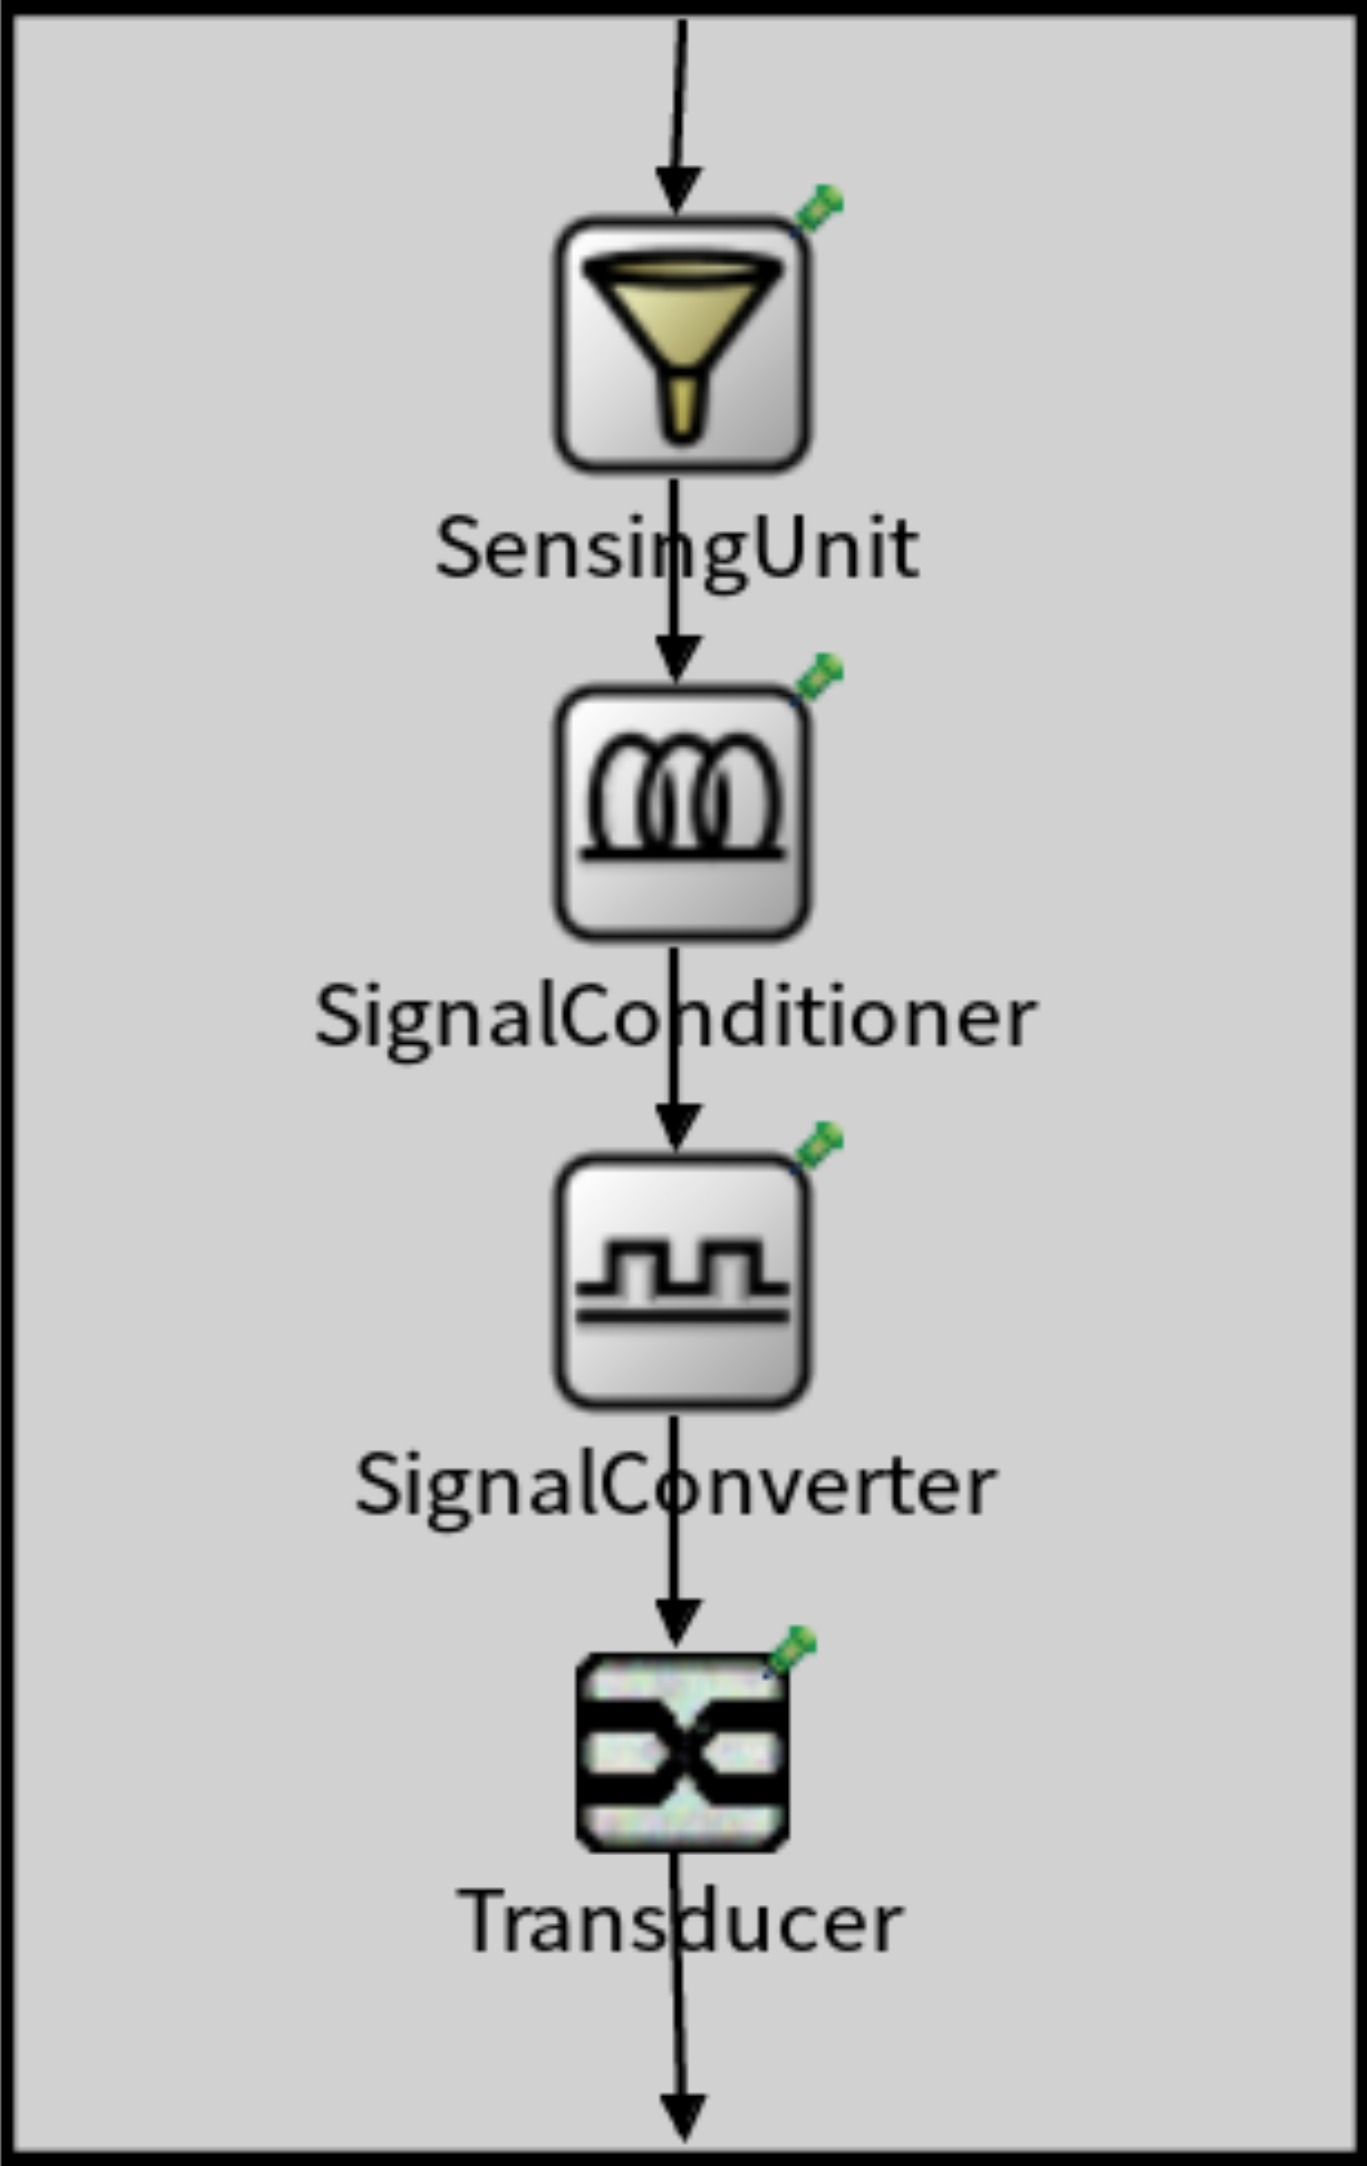
\includegraphics[width=0.3\textwidth]{SensorModel}
\end{figure}

Es liegt ein abstraktes Modul und ein Modulinterface für die verschiedenen Sensoren vor und für jeden Sensortyp existiert ein Sensormodul, welches vom abstrakten Modul erbt und das Sensorinterface implementiert.\\
Die abstrakte Klasse besitzt wenige Parameter; zum einen type, in dem in der jeweiligen Sensorimplementierung der Typ des Sensors definiert werden muss und die beiden Parameter dataBandwidth und controlBandwidth, welche die Bandbreite für die 2 verschiedenen Arten von Channels definieren.\\
Das wichtigste ist natürlich die Definition der Submodule (\ref{lst:AbstractSensor}), denn diese machen die Funktionalität eines Compound Moduls aus. Die Abbildung \ref{fig:SensorModel} zeigt diesen Aufbau in bildlicher Form.

\begin{lstlisting}[language=ned,caption={AbstractSensor},label=lst:AbstractSensor]
submodules:
        SensingUnit: <"SensingUnit"+type> like SensingUnitInterface {
            @display("p=100,50");
        }
        SignalConditioner: <"SignalConditioner"+type> like SignalConditionerInterface {
            @display("p=100,120");
        }
        SignalConverter: <"SignalConverter"+type> like SignalConverterInterface {
            @display("p=100,190");
        }
        Transducer: <"Transducer"+type> like TransducerInterface {
            @display("p=100,260");
        }
\end{lstlisting}

Anhand der Submoduldefinition ist auch ersichtlich, weshalb jedes Modul des Sensors jeweils ein Interface implementieren muss. Für das parametrische Anlegen von Submodulen muss wenigstens ein Interface definiert werden, dem das Modul angehören muss, damit nicht jedes beliebige Modul an dieser Stelle eingesetzt werden kann.

\subsubsection{SensorNode}

\begin{figure}[htbp]
\centering
\caption{Aufbau des Compoundmoduls SensorNode}
\label{fig:Sensornode}
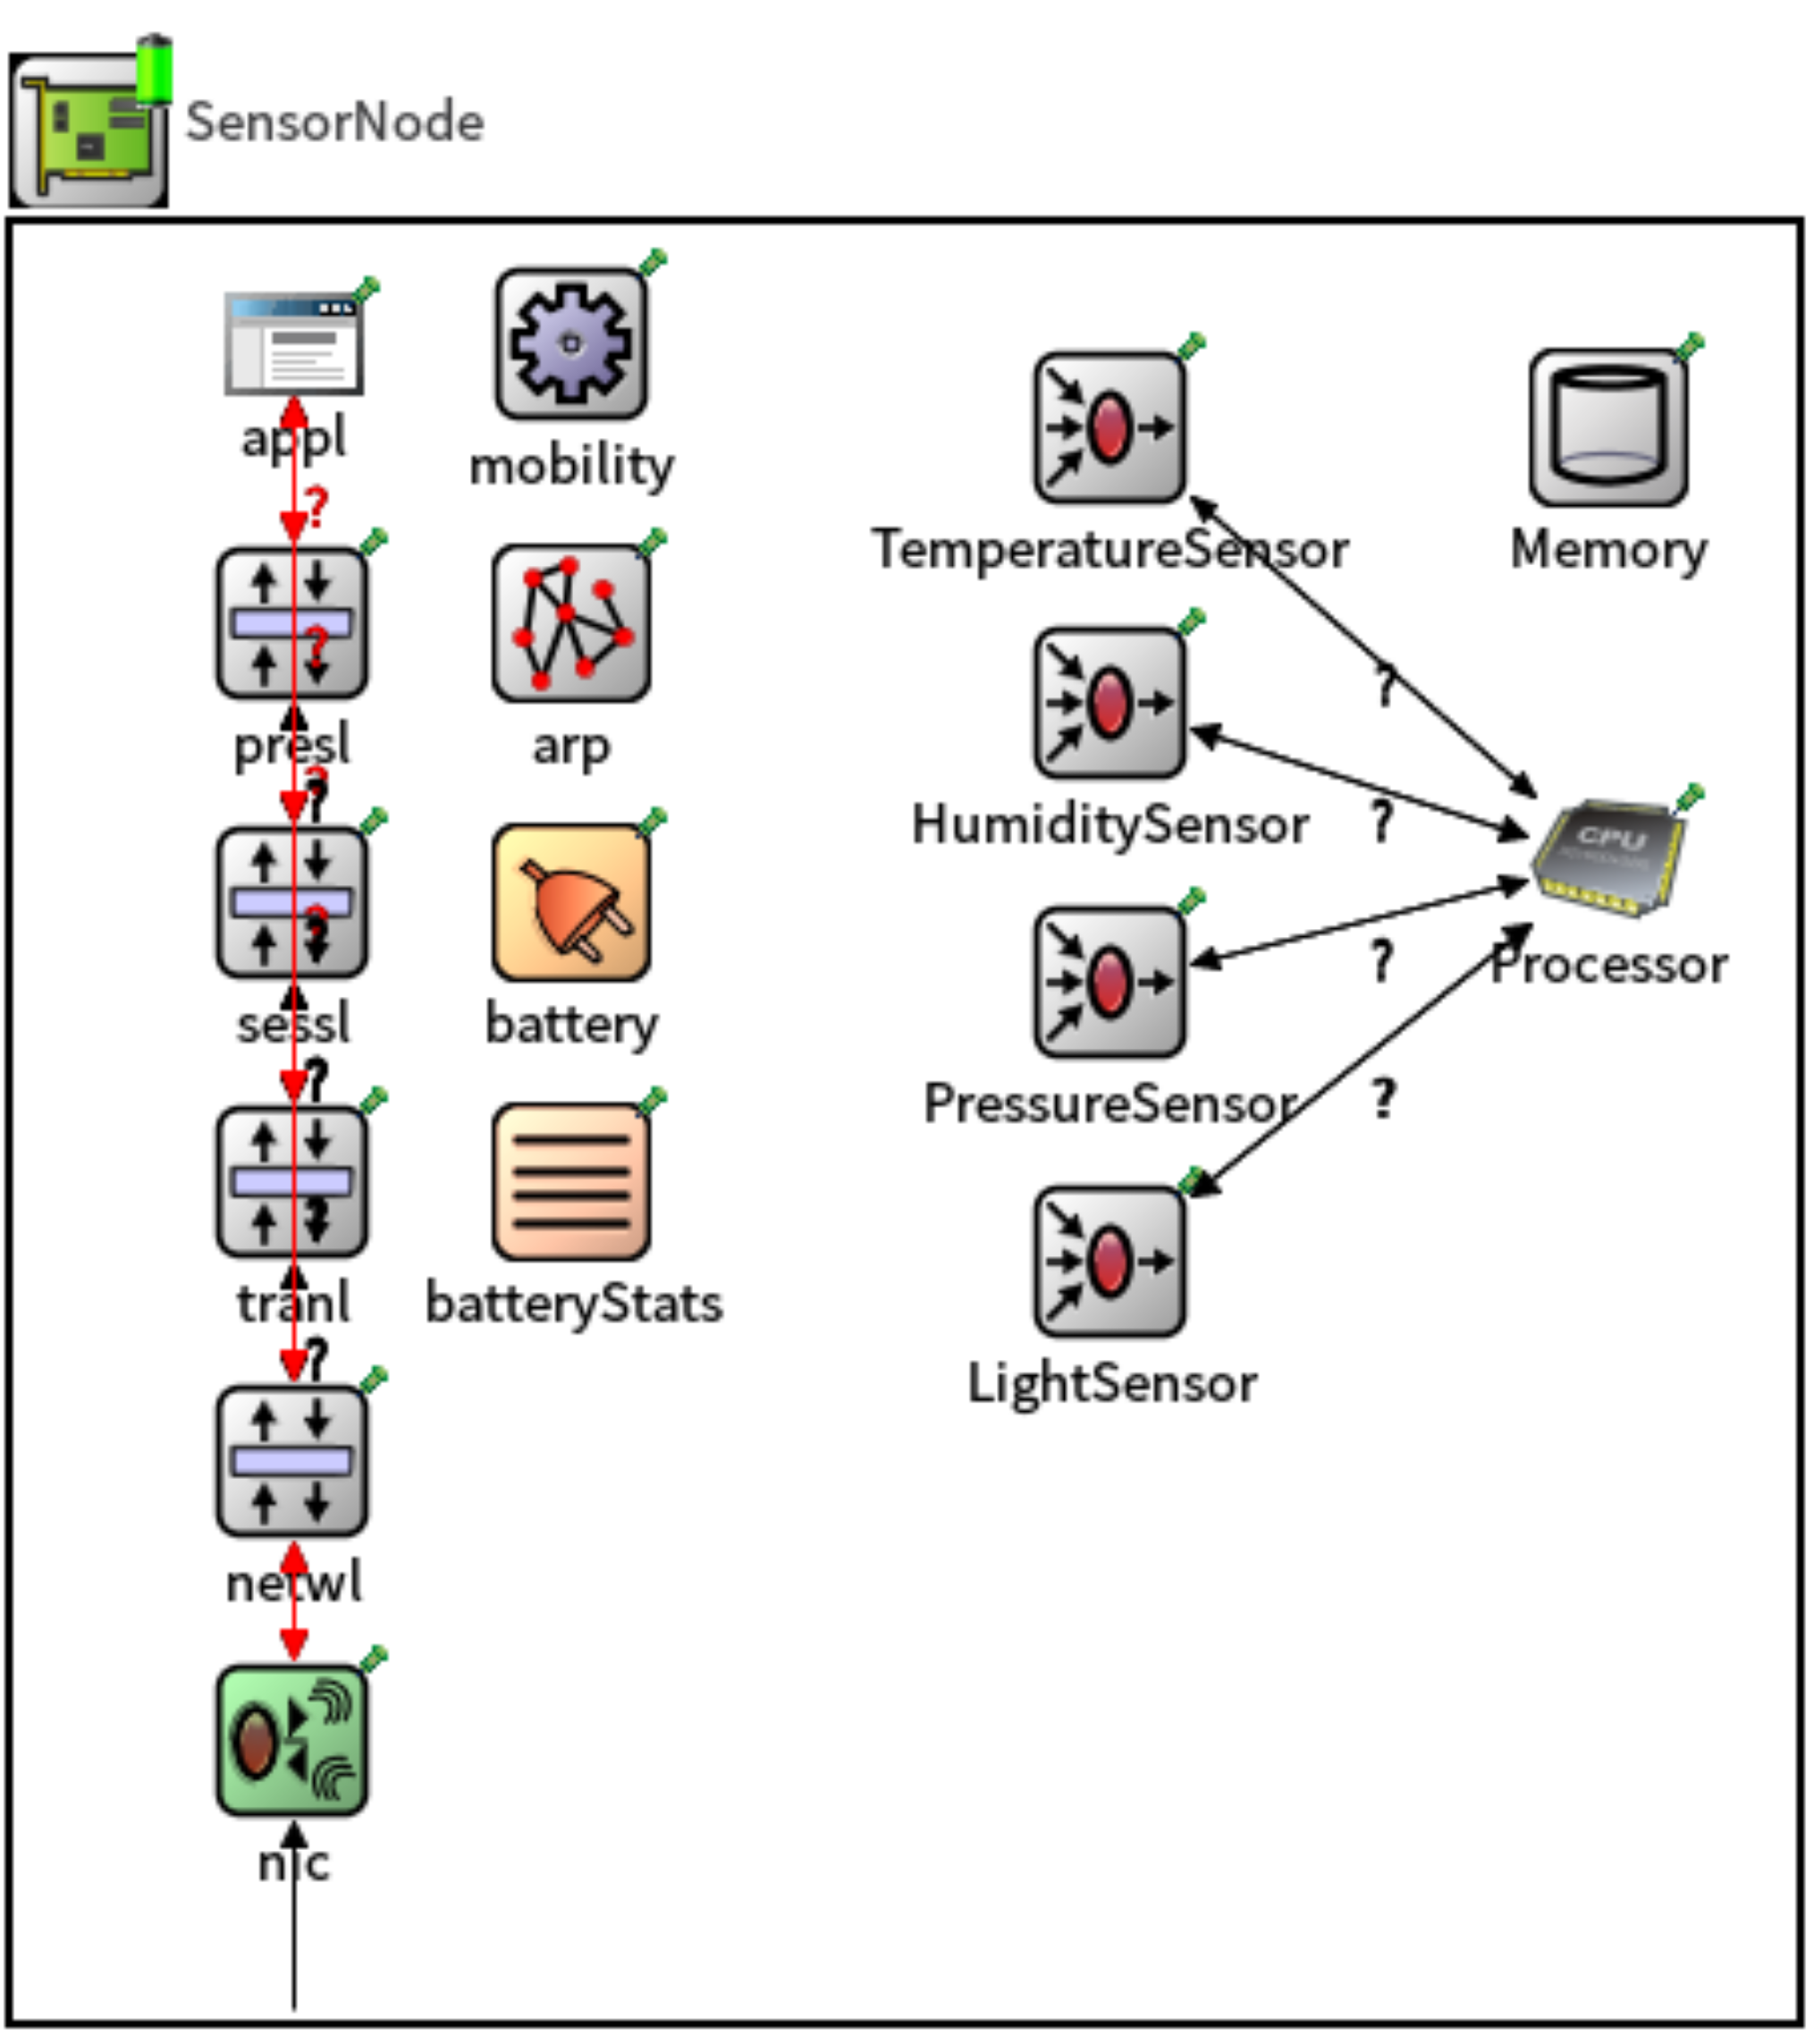
\includegraphics[width=0.7\textwidth]{Sensornode}
\end{figure}

Der SensorNode ist das komplexeste Compound Modul in der Simulation, denn es beinhaltet die bisher beschriebenen Module Sensor, Prozessor, Memory und die in MiXiM enthaltenen Module für die Funkkommunikation und eine Batterie.\\
Die MiXiM-Module werden dem Sensorknoten durch das erben von dem Modul WirelessNodeBatteryPlusTran aus dem MiXiM-Framework zugewiesen, da dieses die benötigte Batterie und die Funkkommunikation bereitstellt. Alle anderen Module werden wie im Beispiel \ref{lst:SensorNode} definiert. Dieses ist dabei auf die Definition der Submodule reduziert.

\begin{lstlisting}[language=ned,caption={SensorNode mit den neu definierten Modulen},label=lst:SensorNode]
module SensorNode extends WirelessNodeBatteryPlusTran like SensorNodeInterface
{
    parameters:
    
        //[...]

    submodules:
        TemperatureSensor: TemperatureSensor if hasTemperatureSensor {
            @display("p=275,51");
            dataBandwidth = dataBandwidth;
            controlBandwidth = controlBandwidth;
        }
        HumiditySensor: HumiditySensor if hasHumiditySensor {
            @display("p=275,120");
            dataBandwidth = dataBandwidth;
            controlBandwidth = controlBandwidth;
        }
        PressureSensor: PressureSensor if hasPressureSensor {
            @display("p=275,190");
            dataBandwidth = dataBandwidth;
            controlBandwidth = controlBandwidth;
        }
        LightSensor: LightSensor if hasLightSensor {
            @display("p=275,260");
            dataBandwidth = dataBandwidth;
            controlBandwidth = controlBandwidth;
        }
        Memory: Memory {
            @display("p=400,51");
        }
        Processor: Processor {
            @display("p=400,159");
        }
        
    connections:
    
        //[...]
        
}        
\end{lstlisting}

Durch das Setzen von hasTemperatureSensor und den analogen booleschen Variablen für die anderen Sensortypen kann für jeden Sensorknoten festgelegt werden, über welche Sensoren er verfügt. Das kann beispielsweise innerhalb der Definition des Netzwerkes geschehen.

\begin{itemize}
\item TemperatureSensor
\item HumiditySensor
\item LightSensor
\item PressureSensor
\end{itemize}

\subsubsection{Messages und Channels}

Nachrichten sind das essenzielle Werkzeug, um in einem Netzwerk Kommunikation zu ermöglichen. Es gibt ein vordefiniertes Modul cMessage, welches dafür genutzt werden kann. Dieses beinhaltet notwendige Informationen wie zum Beispiel Sendermodul und -gate, Empfängermodul und -gate, Sende-, Empfangs- und Erstellzeit und mehr.

\subsubsection{ExtendedMessage}

Die ExtendedMessage erweitert diese Funktionalität um einige Informationen für die Statistik.

\subsubsection{DatarateChannel}

DatarateChannel ist ein von Omnet++ definiertes Modul. Es kann mit verschiedenen Parametern versehen werden, um den jeweiligen Umständen angepasst zu werden. Der Wichtigste ist dabei der double-Wert datarate, welcher in Bit pro Sekunde angegeben wird und festlegt, mit welcher Rate Daten durch den Channel gesendet werden können. Weiterhin kann auch ein delay und eine bit- beziehungsweise packet-error-rate festgelegt werden.\\
In der Simulation wurde dieses Modul genutzt, um die verschiedenen Kanäle für den Datenverkehr und die Steuerungskanäle zu trennen.

\subsubsection{BasicWSN}

Das Netzwerk BasicWSN dient als abstraktes Modul für alle Netzwerke, welche die Sensorikimplementierungen verwenden sollen. Es beinhaltet viele grundlegende Initialisierungen. So wird hier zum Beispiel die Umgebung definiert, welche durch die Klasse CustomWorldUtility beschrieben wird. Für diese werden Werte wie die Playground-Größe gesetzt, sowie einige Standardwerte definiert. So zum Beispiel der Speicherort für die Umgebungswerte.\\
Neu definierte Netzwerke mit Sensorknoten sollten stets von diesem Netzwerk erben. Alle Beispiele dieses Projekts tun dies ebenfalls. 

\subsection{Simulationsparameter und omnetpp.ini}

Die omnetpp.ini ist eine Datei, in der Eigenschaften der Simulation geändert werden können, ohne dass man den Sourcecode bearbeiten und danach neu kompilieren muss. Es bietet sich daher an, alle Variablen und Konstanten, welche sich öfters ändern hier zu definieren. Die entscheidenden Parameter, welche die Eigenschaften der Sensoriksimulation beeinflussen, werden im Folgenden aufgeführt und erläutert.

\begin{itemize}
\item Energieverwaltung - kann global oder auch für jedes Modul einzeln definiert werden
\begin{itemize}
\item currentConsumption - integer (in mA): Verbrauch über Zeit
\item energyConsumption - integer (in mWs): Verbrauch für eine Operation
\end{itemize}
\item Energieverwaltung - Prozessorspezifisch, Energieverbrauch für die verschiedenen Prozessormodi
\begin{itemize}
\item currentConsumptionNormal - integer (in mA)
\item energyConsumptionNormal - integer (in mWs)
\item currentConsumptionPowerSaving - integer (in mA)
\item energyConsumptionPowerSaving - integer (in mWs)
\item currentConsumptionHighPerformance - integer (in mA)
\item energyConsumptionHighPerformance - integer (in mWs)
\end{itemize}
\item Energieverwaltung - die folgenden Parameter gelten für die Peripheriemodule (also alle außer dem Prozessor)
\begin{itemize}
\item normalRatio - double: Verhältnis von currentConsumption und energyConsumption im normalen Modus
\item powerSavingRatio - double: Verhältnis von currentConsumption und energyConsumption im power saving Modus
\item highPerformanceRatio - double: Verhältnis von currentConsumption und energyConsumption im high performance Modus
\item battery.nominal - double (in mAh): Akkukapazität
\end{itemize}
\item Metadaten/Eventintervalle - alle Events können komplett deaktiviert werden, indem der Wert auf 0 gesetzt wird
\begin{itemize}
\item dataGranularity - integer: je größer der Wert gewählt wird, um so grober ist die Berechnung der Sensorwerte, beim Werte n wird für einen Würfel der Seitenlänge = n jeweils 1 Messwert generiert
\item sensingIntervall - integer (in s): mit welchem Zeitabstand Messungen werden durchgeführt
\item shiftProcessorModeNormalIntervall - integer (in s): wie lange wird der Prozessormodus normal behalten, bevor wieder gewechselt wird
\item shiftProcessorModePowerSavingIntervall - integer (in s): wie lange wird der Prozessormodus power saving behalten, bevor wieder gewechselt wird
\item shiftProcessorModeHighPerformanceIntervall - integer (in s): wie lange wird der Prozessormodus high performace behalten, bevor wieder gewechselt wird
\item collectStatisticsIntervall - integer (in s): mit welchem Zeitabstand werden statistische Daten gemessen
\item readAndClearStorageIntervall - integer (in s): mit welchem Zeitabstand wird der Memory ausgelesen und geleert
\item dataRecreationIntervall - integer (in s): mit welchem Zeitabstand werden neue Umgebungswerte generiert
\end{itemize}
\item Netzwerkparameter
\begin{itemize}
\item createData - boolean: beim Start der Simulation neue Messwerte generieren
\item numHosts - integer: wie viele Sensorknoten befinden sich in der Simulation
\item noisyWorld - boolean: wenn auf true gesetzt, macht die Umwelt einige Ausgaben mit Informationen über Zustand und durchgeführte Aktionen
\item noisy - boolean: wenn auf true gesetzt, macht der Sensorknoten einige Ausgaben mit Informationen über Zustand und durchgeführte Aktionen
\item playgroundSizeX - integer (in m): Größe der X-dimension
\item playgroundSizeY - integer (in m): Größe der Y-dimension
\item playgroundSizeZ - integer (in m): Größe der Z-dimension
\end{itemize}
\item Sensorknoten
\begin{itemize}
\item dataBandwidth - double (in bps): Bandbreite mit der Daten innerhalb des Sensorknotens versendet werden
\item controlBandwidth - double (in bps): Bandbreite mit der die Steuerungsleitungen des Prozessors senden
\item Memory.storageSize - integer: definiert die Anzahl von Datensätze, die das Memorymodul parallel speichern kann
\end{itemize}
\end{itemize}

\section{Funktionsweise mit Beispielanwendungen}

All die in diesem Kapitel beschriebenen Module wirken für die Simulation zusammen, um ein Netzwerk aus Sensorknoten zu schaffen, in dem die Knoten miteinander und mit ihrer Umgebung gemeinsam agieren können. Dazu werden nach dem Start der Simulation Umweltparameter bereitgestellt und eine festgelegte Anzahl von verschiedenen Sensorknoten erzeugt. Diese können sich anschließend bewegen oder ihr Position beibehalten. Sie können mit ihren Sensoren Werte der Umgebung erfassen und diese über Funk an andere Sensorknoten übertragen, sollte diese in der näheren Umgebung zur Verfügung stehen.

\subsection*{allgemeine Beispiele}

Die allgemeinen Beispiele zeigen auf, wie einfache Anwendungen unter Nutzung der Sensorknoten aussehen könnten. Dabei werden einfache Netzwerke mit unterschiedlichen Knoten gezeigt, und wie diese erzeugt werden können.

\paragraph{BasicExample}

Das Netzwerk BasicExample beinhaltet einige verschiedene Typen von Sensorknoten. Zur Verwendung von der Sensorik sollte das Netzwerk vom Modul BasicWSN erben, welches schon viele Parameter initialisiert, die für das korrekte Funktionieren notwendig sind. Alle weiteren Parameter, welche in der omnet.ini definiert sind, dienen dazu, die Simulation entsprechend des gewünschten Verhaltens anzupassen, wie zum Beispiel Batteriekapazität, Energieverbrauch einzelner Module und so weiter.

\paragraph{AllNodes}

AllNodes ist ein Beispielnetzwerk, in dem alle möglichen Kombinationen von Sensorknoten vorgeführt werden. Aus den 4 verschiedenen Sensortypen können 15 verschiedene Arten von Sensorknoten erzeugt werden, wenn man den Knoten ohne jeglichen Sensor nicht mitzählt, welcher in diesem Netzwerk aber ebenfalls vorhanden ist. Das Beispiel dient zum Testen aller verschiedener Kombinationsmöglichkeiten, da sich die einzelnen Implementierungen leicht voneinander unterscheiden.

\paragraph{TrafficGenExample}

Das Netzwerk TrafficGenExample unterscheidet nur wenig vom BasicExample. Der entscheidende Unterschied ist, dass hierbei ein anderes Modul aus dem ApplicationLayer von MiXiM genutzt wurde, nämlich TrafficGen. Dieses kann sehr viele Nachrichten generieren und so den Kommunikationsverkehr sehr gut testen.

\paragraph{SensorExample}

Im Beispiel SensorExample wird die Funktionsweise von den Bauelementen der simulierten Sensorik und der Umgebung aufgezeigt. Dafür wurden verschiedene Parameter in der omnet.ini und in den Modulen so gewählt, damit dies gut abgelesen werden kann (Listing \ref{lst:sePar}).\\

\begin{lstlisting}[language=ned,caption={Parameter für das Beispiel SensorExample},label=lst:sePar]
**.sensingIntervall = 10000s
**.shiftProcessorModeNormalIntervall = 3000s
**.shiftProcessorModePowerSavingIntervall = 3000s
**.shiftProcessorModeHighPerformanceIntervall = 3000s
**.collectStatisticsIntervall = 1700s
**.readAndClearStorageIntervall = 34000s
**.dataRecreationIntervall = 13000s
**.noisyWorld = true;
**.noisy = true; 
\end{lstlisting}

Die beiden Parameter noisy und noisyWorld dienen dazu, dass während der Simulation an den entscheidenden Stellen der Simulation Ausgaben gemacht werden. Diese geben Informationen darüber, welche Aktionen ausgeführt werden und wie der Zustand von einigen Modulen ist, so zum Beispiel wird bei Änderung der Speicherinhalt vom Memory ausgegeben und stets der aktuelle Prozessormodus angegeben.\\
Im Beispiel wird alle 10000 Sekunden von den Sensoren ein Messwert abgegriffen. Außerdem werden die vorliegenden Werte alle 13000 Sekunden geändert. Die verschiedenen Werte werden dann nacheinander im Memory abgelegt.\\
\begin{lstlisting}[language=ned,caption={Ausgabe vom Prozessor bei t=40000s},label=lst:seProzessorOut]
Processor: received data:
Processor: Temperature: 10 (t=0s)
Processor: Temperature: 10 (t=10000s)
Processor: Temperature: 11 (t=20000s)
Processor: Temperature: 27 (t=30000s)
\end{lstlisting}
Da der Speicher im Beispiel nur Platz für 4 Datensätze bietet und auch nur ein einziger Sensor genutzt wird ist er nach 4 Messungen voll. Daher wird alle 34000 Sekunden, also nach jeweils 4 Messungen, der Speicher geleert. Die bis dahin gespeicherten Werte werden dann an den Prozessor gesendet. Eine Beispielausgabe des Prozessors aus einem Testlauf, in dem in dem nur ein einziger Knoten mit einem Temperatursensor genutzt wurde, sind in Listing \ref{lst:seProzessorOut} zu sehen. Diese Ausgabe wurde zum Zeitpunkt t=34000s getätigt, ausgelöst durch den Event readAndClearStorage. Es wurde also gleichzeitig auch der Memory gelöscht. Direkt danach wurde der Speicher wieder mit neuen Datensätzen gefüllt.\\
In der Realität ist dies ein realistisches Szenario. Während sich die Knoten in einem Ruhemodus befinden, um Strom zu sparen, kann dennoch regelmäßig eine Messung durchgeführt und gespeichert werden. Wenn nun ein Zeitfenster erreicht wird, in dem Kommunikation im Netzwerk stattfindet, so werden gleich mehrere Messwerte auf einmal versendet.

\begin{figure}[htbp]
\centering
\caption{Die verschiedenen Events im Beispiel SensorExample}
\label{fig:seEvents}
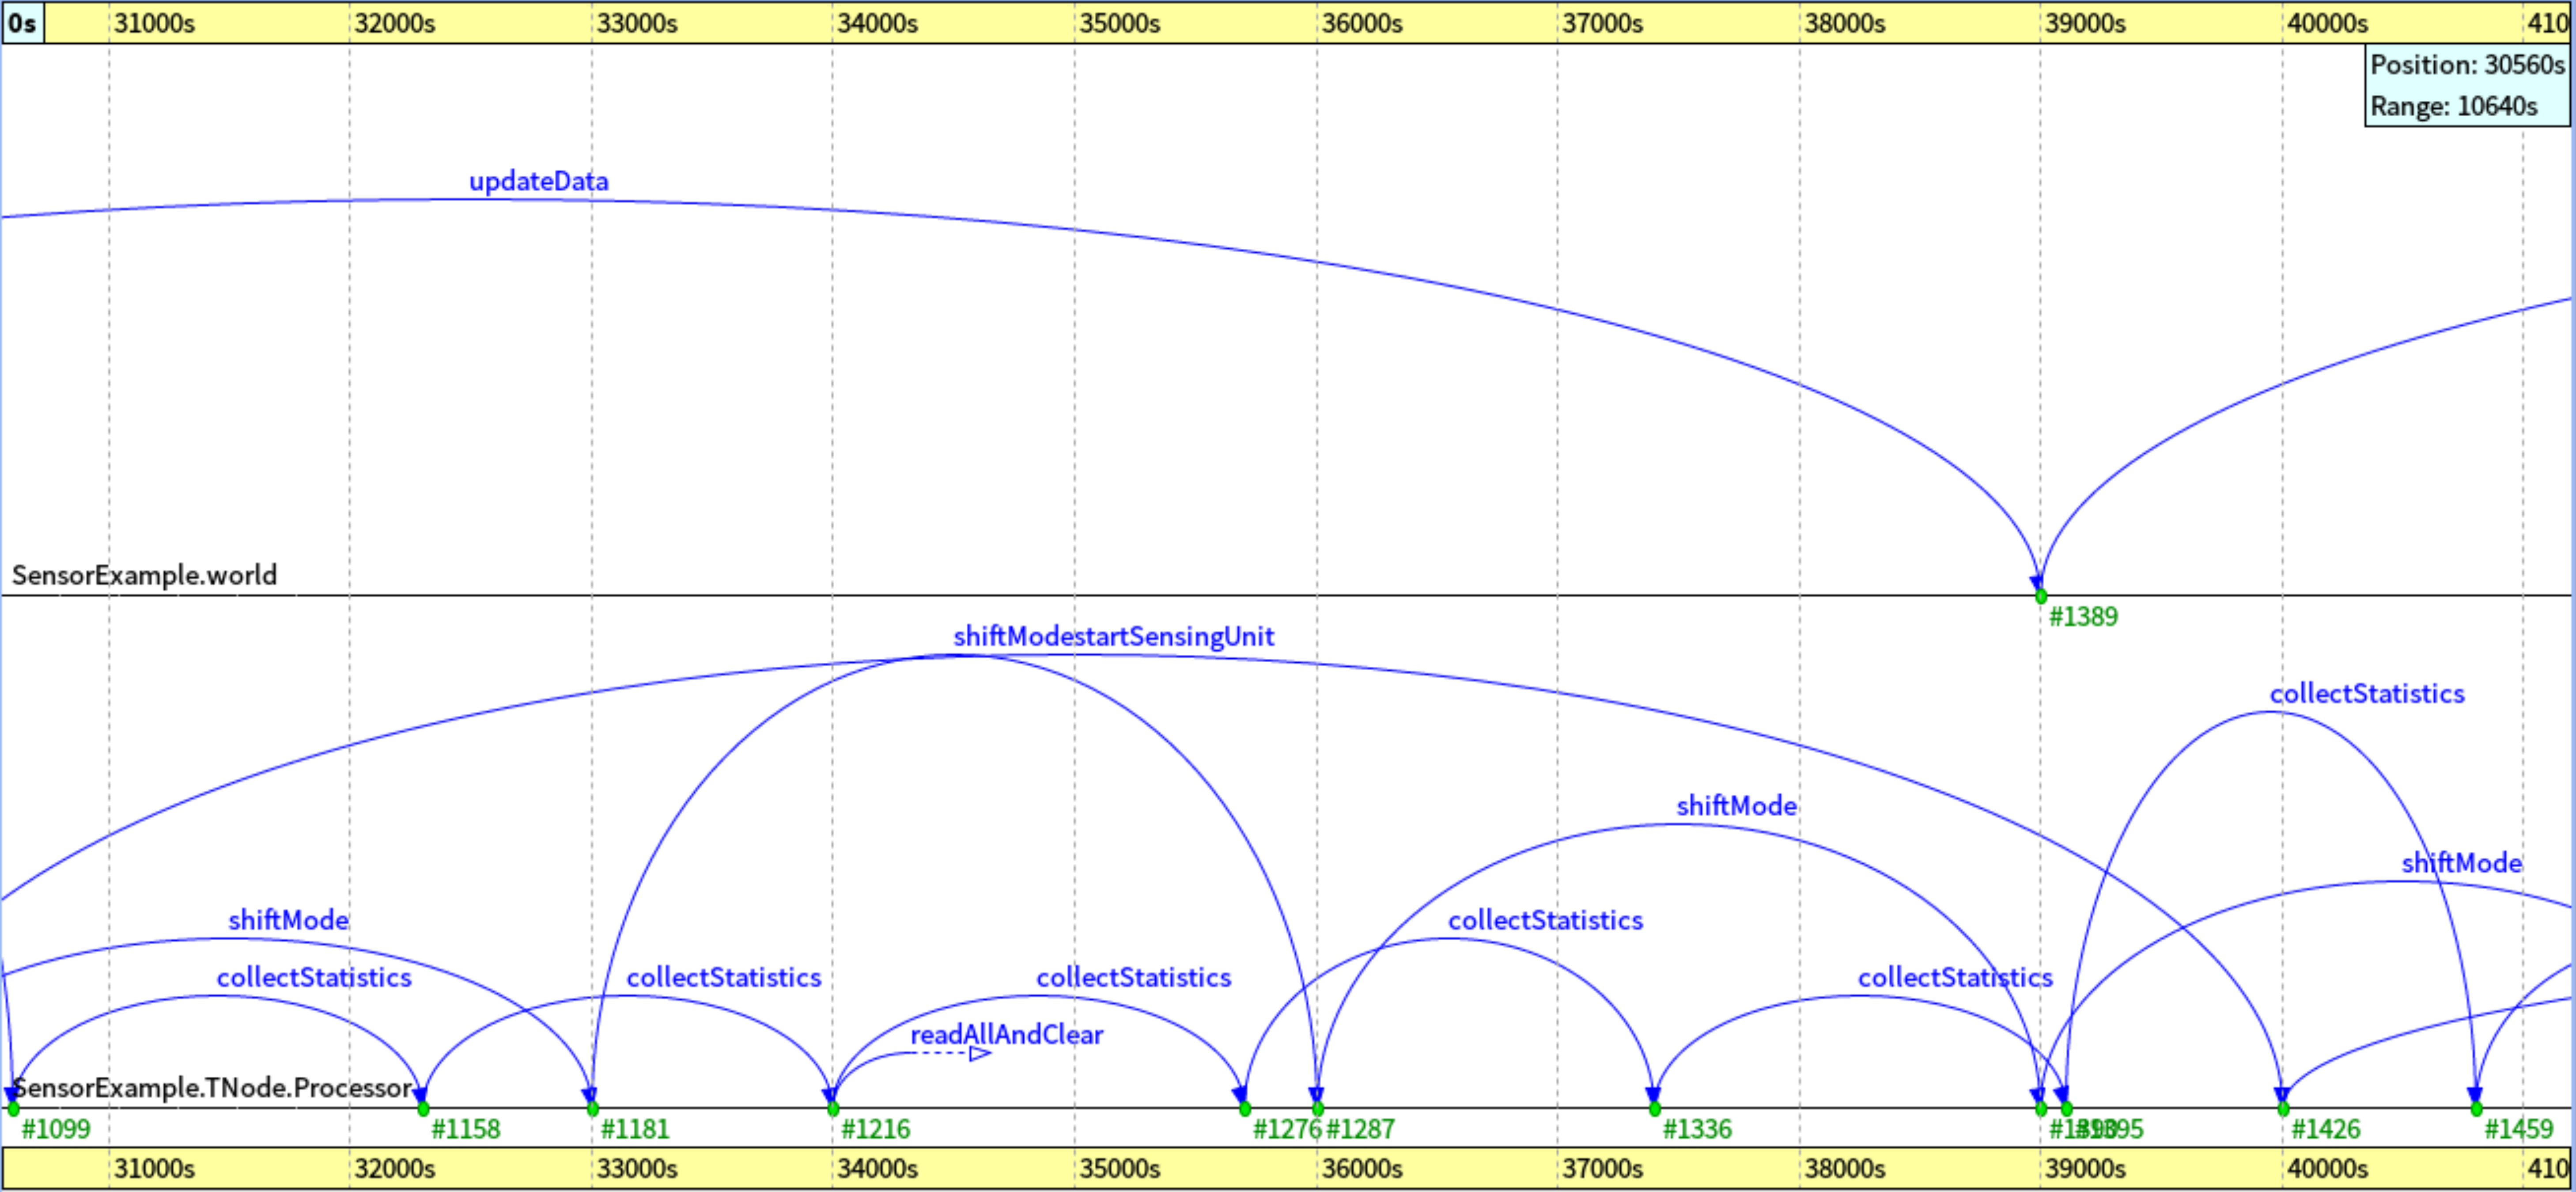
\includegraphics[width=\textwidth]{sensorExampleEvents}
\end{figure}

\begin{figure}[htbp]
\centering
\caption{Beispiel für den Nachrichtenverlauf beim Einlesen von Sensordaten}
\label{fig:seStartMeasuring}
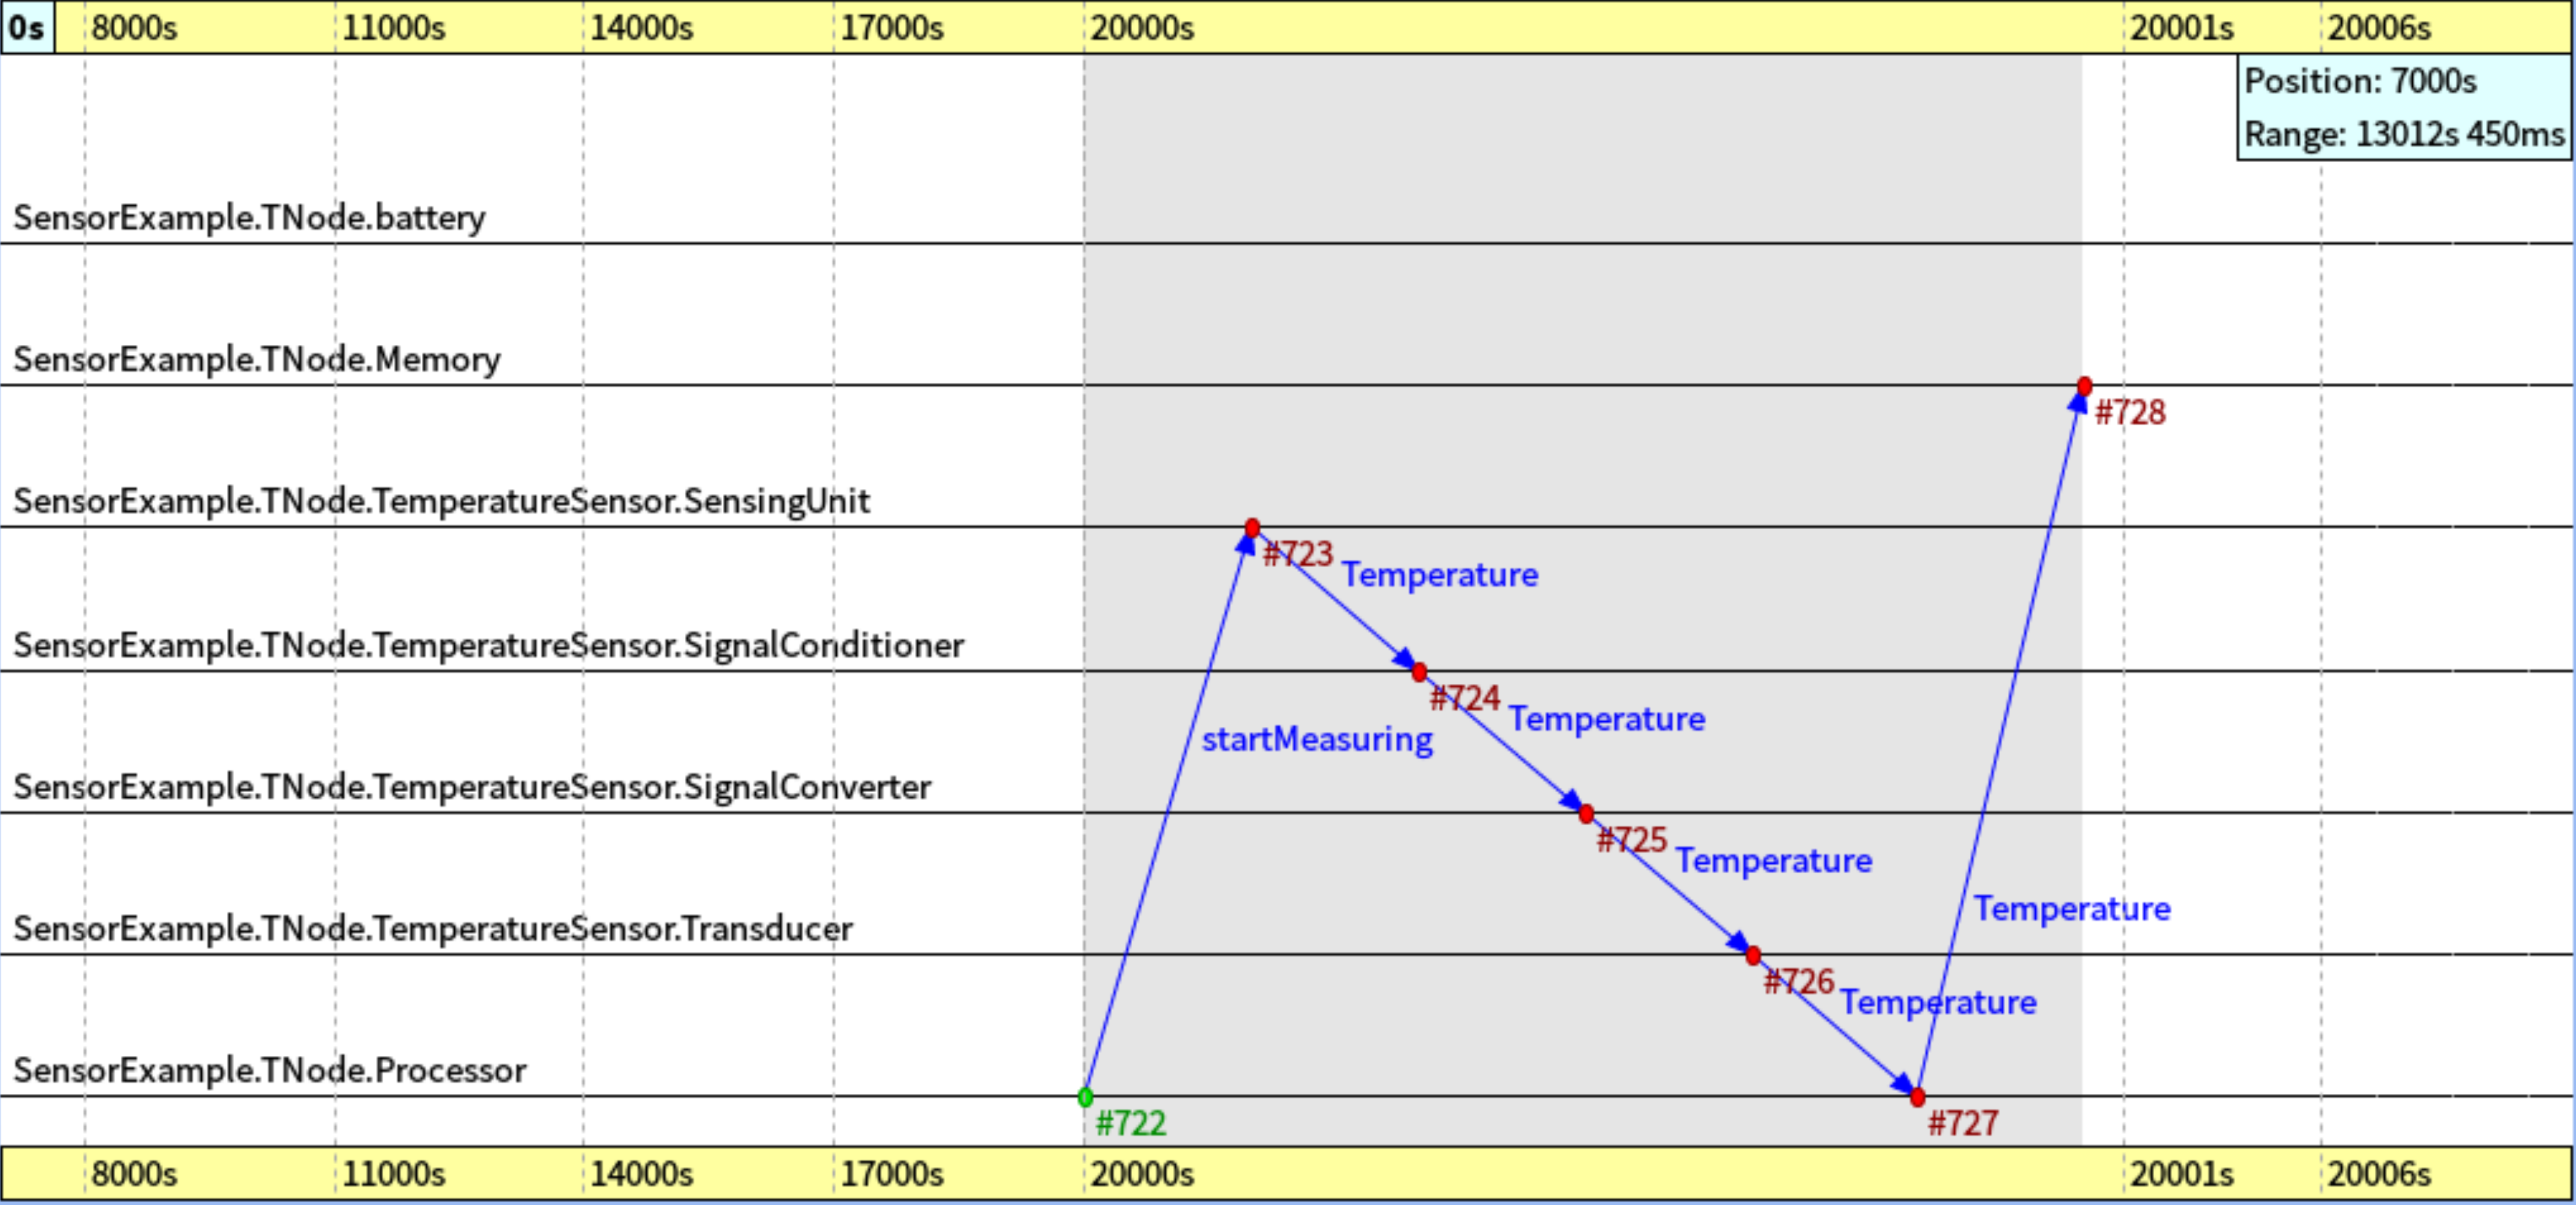
\includegraphics[width=\textwidth]{startMeasuring}
\end{figure}

Im Bild \ref{fig:seEvents} sind die verschiedenen Events zu sehen, die im Sensor- und Worldmodul auftauchen. In der CustomWorldUtility wird nur einer der Events ausgelöst, welcher zum erneuten Erstellen von Sensordaten dient: updateData mit dem Intervall dataRecreationIntervall.\\
Die anderen Events finden im Prozessor statt. Sie dienen dazu bestimmte Arbeitsabläufe anzustoßen. Der wichtigste Event ist wohl startSensingUnit, dessen Zeitintervall durch sensingIntervall festgelegt wird. Er dient dazu, einen Messvorgang in Gang zu setzen. Am Ende werden die gemessenen Werte stets im Memory gespeichert.

\begin{itemize}
\item startSensingUnit
\begin{itemize}
\item sensingIntervall
\end{itemize}
\item shiftMode
\begin{itemize}
\item shiftProcessorModeNormalIntervall
\item shiftProcessorModePowerSavingIntervall
\item shiftProcessorModeHighPerformanceIntervall
\end{itemize}
\item collectStatistics
\begin{itemize}
\item collectStatisticsIntervall
\end{itemize}
\item readAllAndClear
\begin{itemize}
\item readAndClearStorageIntervall
\end{itemize}
\item updateData
\begin{itemize}
\item dataRecreationIntervall
\end{itemize}
\end{itemize}

In Bild \ref{fig:seStartMeasuring} ist der Nachrichtenverlauf zu sehen, welcher durch den Event startMeasuring ausgelöst wird. Der Event wird innerhalb des Prozessormoduls gestartet. Dort wird anschließend eine Nachricht an die SensingUnits der zugehörigen Sensoren geschickt. Innerhalb der SensingUnit wird dann eine Messung durchgeführt. Diese Messdaten werden dann wiederum durch die verschiedenen Module des Sensor geleitet. Zuerst zum SignalConditioner, zum SignalConverter und zuletzt zum Transducer. Nachdem diese Stationen durchlaufen wurden, wird der fertige Messwert zurück zum Prozessor gesendet. Dieser speichert dann zunächst den Wert im Memory ab.

\subsection*{spezielles Verhalten}

Im folgenden Abschnitt werden einige speziellere Netzwerke, als die bisherigen beschrieben. Diese führen nicht nur stupide Kommunikationen durch, sondern testen außerdem die verschiedenen Prozessormodi und zeigen, wie diese die Lebenszeit eines Knotens beeinflussen können.

\paragraph{SleepVsNoSleep}

\begin{figure}[htbp]
\centering
\caption{Powermodi im Beispiel SleepVsNoSleep}
\label{fig:sleepVsNoSleepPowerModes}
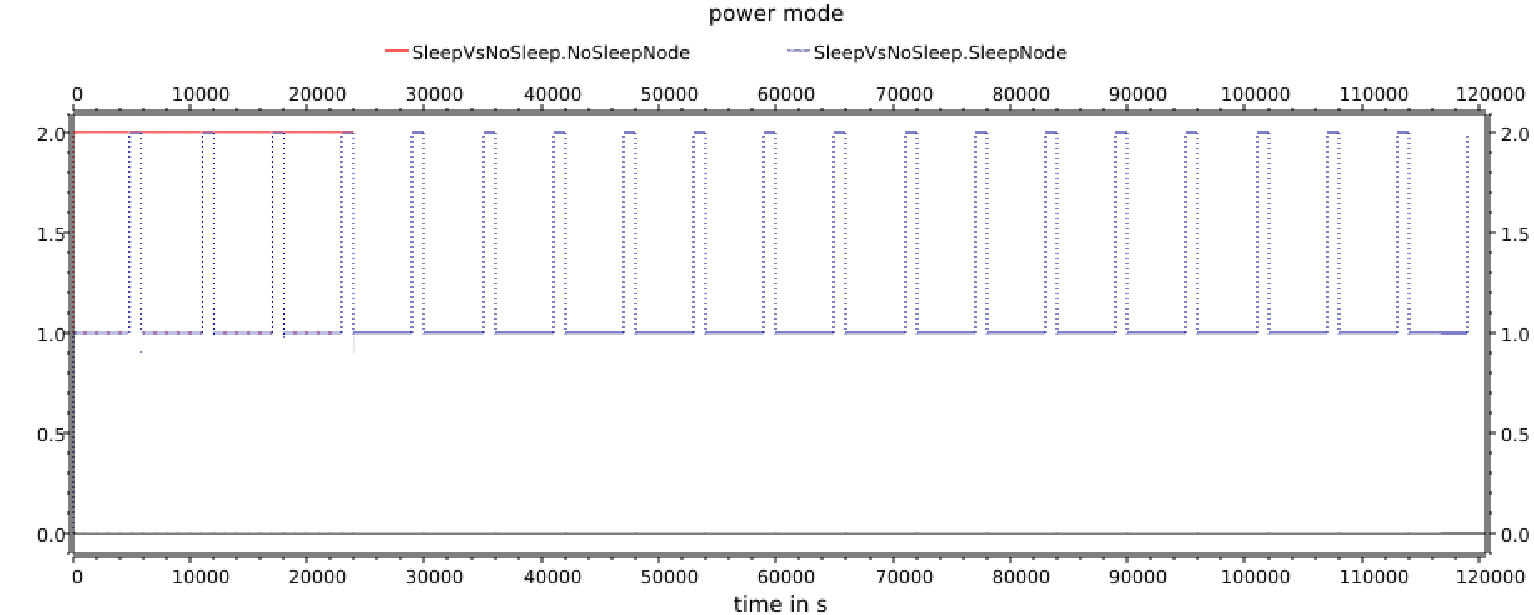
\includegraphics[width=\textwidth]{sleepVsNoSleepPowerModes}
\end{figure}

\begin{figure}[htbp]
\centering
\caption{Ladezustand im Beispiel SleepVsNoSleep}
\label{fig:sleepVsNoSleepResRel}
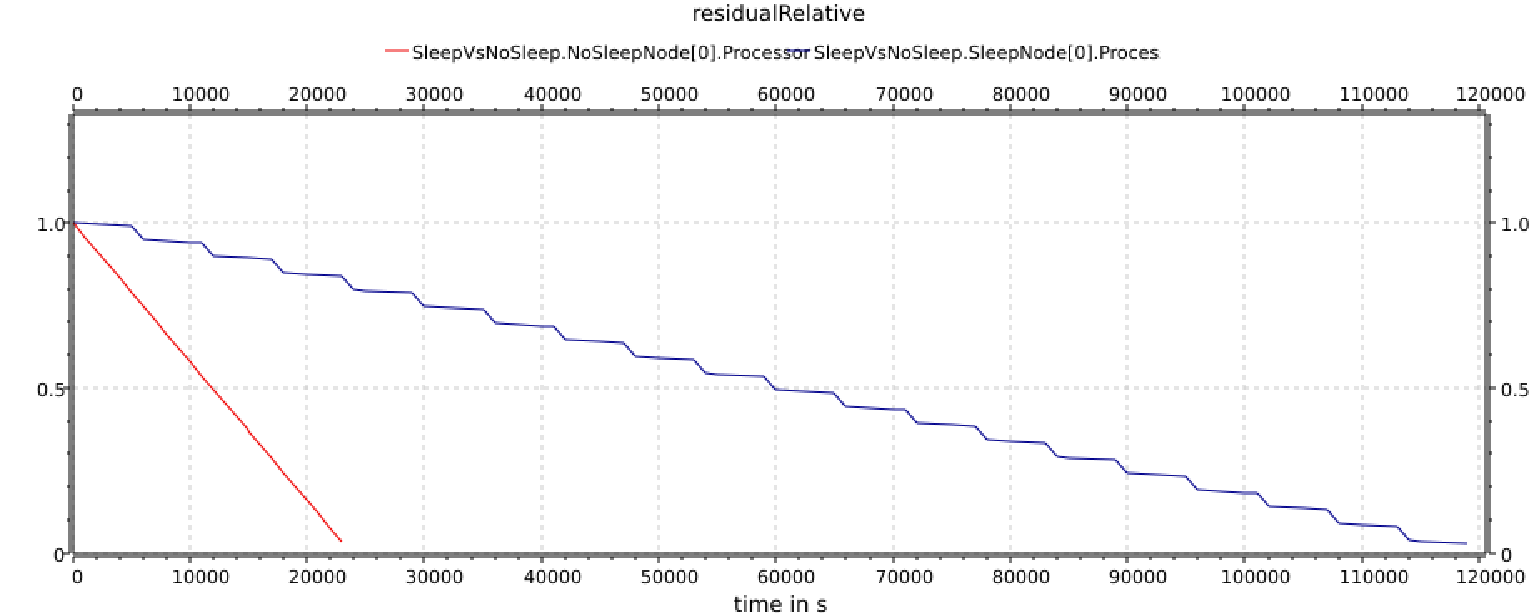
\includegraphics[width=\textwidth]{sleepVsNoSleepResRel}
\end{figure}

Im Netzwerk SleepVsNoSleep befinden sich 2 beinahe identische Knoten. Die Bauteile auf beiden sind die selben, der einzige Unterschied besteht darin, dass einer der beiden Knoten nur einen Energiemodus benutzt, in dem ganz normal Energie im Stand-by-Modus verbraucht wird. Im Gegensatz dazu kann der andere Knoten zwischen 3 verschiedenen Modi zyklisch wechseln, wobei er in jedem dritten Intervall in einen schlafenden Zustand übergeht, bei dem deutlich Energie gespart werden kann.\\
Die Abbildung \ref{fig:sleepVsNoSleepPowerModes} zeigt die verschiedenen Powermodi. Dabei ist entscheidend, dass der Energiesparmodus durch den Wert 1 repräsentiert wird. Der rote Knoten wechselt in diesem Beispiel niemals in den Energiesparmodus, sondern bleibt während der gesamten Zeit in einem Modus. Der andere Knoten wechselt jeweils für 5000 Sekunden in den Energiesparmodus. Nur dazwischen wechselt er immer für kurze Zeit in einen aktiven Modus.\\
Das Resultat ist in Abbildung \ref{fig:sleepVsNoSleepResRel} sofort ersichtlich. Der rote Knoten, welcher nie in den schlafenden Modus wechselt, hat eine erheblich kleinere Lebenszeit. Das Verhältnis der Lebenszeit ist natürlich davon abhängig, wie viel Energie durch den Energiesparmodus gespart werden kann.

\paragraph{SleepOutOfSync}

\begin{figure}[htbp]
\centering
\caption{Powermodi im Beispiel SleepOutOfSync}
\label{fig:sleepOutOfSyncModes}
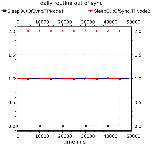
\includegraphics[width=\textwidth]{outOfSync}
\end{figure}

Das Beispiel namens SleepOutOfSync zeigt ebenso wie SleepVsNoSleep die Verwendung der Prozessor-Energie-Modi. Allerdings wird bei diesem Beispiel gezeigt, warum der Wach-und-Schlaf-Zyklus von den verschiedenen Knoten, welche sich in einem Sensornetzwerk befinden zeitlich aufeinander abgestimmt werden muss.\\
Dazu ist lediglich ein kleines Netzwerk von 2 Knoten vorhanden, welche genau zeitversetzt zwischen dem Energiesparmodus, in dem nichts gesendet oder empfangen werden kann und einem normal Modus wechseln. In dieser extremen Variante würde das Netzwerk gar nicht erst vorhanden sein, da beide Knoten niemals von der Existenz des jeweils anderen erfahren würden.\\
Das zeigt, weshalb verschiedene Knoten eines Netzwerkes in der Praxis einen synchronen Wach-und-Schlaf-Zyklen besitzen müssen, damit keine unnötige Kommunikation stattfindet, an der nicht alle Knoten beteiligt sind.\\
In Abbildung \ref{fig:sleepOutOfSyncModes} ist dieser Ablauf visualisiert. Dabei kann im Modus mit dem Wert 1 keine Kommunikation stattfinden. Wie man sehen kann, wechseln sich die beiden Knoten genau zwischen aktiven und inaktiven Modi ab. Es kann dadurch zu keiner Kommunikation kommen.